\subsection{Ejercicio 10}
\graphicspath{ {img/10} }

En la actualidad el certificado de persona física de la FNMT no permite su uso para cifrar conversaciones de correo electrónico. Como alternativa podemos generar nuestro propio certificado o utilizar uno de alguna CA reconocida. Decidimos generar nuestros propios certificados firmados por una CA también nuestra con \texttt{openssl}, ya que nos parecía la opción más didáctica.

\subsubsection{Generación de una CA con OpenSSL}

Para crear una CA necesitamos dos cosas, la clave con la que la CA firmara las peticiones de certificado y un certificado público para la CA del que los clientes se puedan fiar para validar los certificados que hayamos firmado.

Decidimos utilizar una clave RSA de 4096 bits. Con el siguiente comando generamos la clave privada de la misma y la almacenamos cifrada con DES:

\begin{minted}[
    frame=single,
    framesep=8pt,
    breaklines,
    bgcolor=bgGray
]{bash}
    openssl genrsa -des3 -out ca.key 4096
\end{minted}

Una vez generada la clave privada, necesitamos un certificado con la clave pública de la CA. Un formato común para compartir las claves públicas junto con su identidad es x509. Con esto, el certificado contiene información sobre la CA y la clave pública. La información puede ser variada, y algunos parámetros habituales son los que pide \texttt{openssl} de manera interactiva al generar el certificado

\begin{minted}[
    frame=single,
    framesep=8pt,
    breaklines,
    bgcolor=bgGray
]{bash}
    openssl req -new -x509 -days 1826 -key ca.key -out ca.crt
\end{minted}

Este comando genera el certificado en formato x509 para la clave \texttt{ca.key}. Indicamos que queremos que tenga una validez de 1826 días (5 años) y que se almacene en \texttt{ca.crt}.

Ahora tenemos una CA que podemos compartir con todos nuestros amigos para que añadan en sus ordenadores (si se fían de nosotros).

\begin{figure}[H]
    \centering
    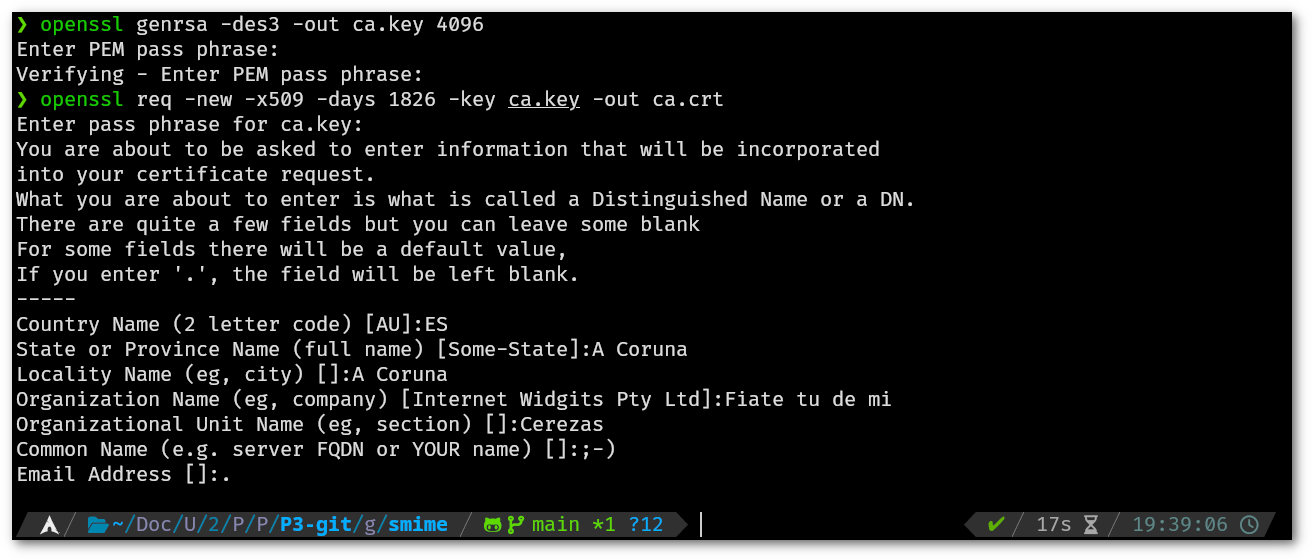
\includegraphics[width=\textwidth]{openssl-ca-sombra.png}
    \caption{Generación de una CA con \texttt{openssl}}
\end{figure}

\subsubsection{Generación de certificados}

Con la CA en funcionamiento necesitamos generar certificados para nuestros usuarios. Esto tiene dos partes:

\begin{itemize}
    \item Generación de una petición de certificado por parte del usuario
    \item Generación de un certificado firmado por la CA
\end{itemize}

Es decir, igual que con la CA, el usuario genera una clave privada pero, en este caso, en lugar de generar su propio certificado de clave pública, genera con su parte privada una \textit{petición de certificado}. A continuación, la CA genera con esta información el certificado correspondiente. De esta forma, el usuario obtiene un certificado público firmado por la Autoridad Certificadora sin tener que compartir nunca su clave privada.

La clave privada del usuario será igual que la de la CA, RSA de 4096 cifrada con DES para su almacenamiento seguro, por lo que se puede generar con el mismo comando:

\begin{minted}[
    frame=single,
    framesep=8pt,
    breaklines,
    bgcolor=bgGray
]{bash}
    openssl genrsa -des3 -out iago.rivas.key 4096
\end{minted}

A continuación se genera la petición de certificado CSR \textit{Certificate Signing Request} con \texttt{openssl}

\begin{minted}[
    frame=single,
    framesep=8pt,
    breaklines,
    bgcolor=bgGray
]{bash}
    openssl req -new -key iago.rivas.key -out iago.rivas.csr
\end{minted}

Con esta petición, la autoridad puede firmar el certificado y devolvérselo al usuario para que lo comparta como su clave pulica. Esto se puede hacer con el siguiente comando en \texttt{openssl}:

\begin{figure}[H]
    \centering
    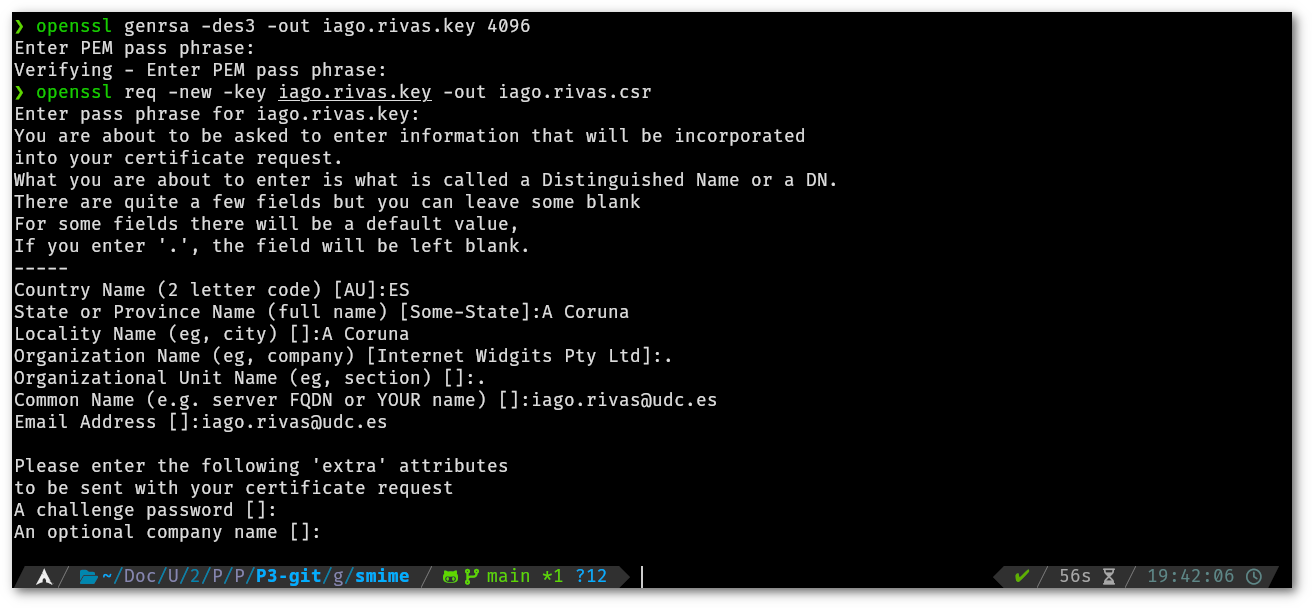
\includegraphics[width=\textwidth]{openssl-key-sombra.png}
    \caption{Generación de la petición de certificado con \texttt{openssl}}
\end{figure}

\begin{minted}[
    frame=single,
    framesep=8pt,
    breaklines,
    bgcolor=bgGray
]{bash}
    openssl x509 -req -days 730 -in iago.rivas.csr -CA ca.crt -CAkey ca.key -set_serial 0xBEEF -out iago.rivas.crt
\end{minted}

Todos los parámetros del certificado los definió el usuario al generar la petición, sin embargo hay algunas cosas que decide la CA, concretamente la duración del certificado, en este caso 730 días (2 años), el número de serie y las características del certificado, en este caso se permite su uso para el correo electrónico, pero se prohibe utilizarlo para cualquier tipo de autenticación.

Para generar el certificado es necesaria la clave privada de la CA, ya que se incluye la firma de la misma para darle validez ante aquellas personas que se fíen de la Autoridad pero no del usuario del certificado.

\subsubsection{S/MIME en Thunderbird}

Para utilizar nuestro certificado S/MIME en Thunderbird tenemos que añadir primero el certificado de la Autoirdad Certificadora y a continuación nuestro certificado. Necesitamos incluír la parte privada, ya que lo usaremos para firmar y descifrar mensajes, por lo que lo exportaremos en el formato PKCS12 también con openssl, utilizando el comando

\begin{minted}[
    frame=single,
    framesep=8pt,
    breaklines,
    bgcolor=bgGray
]{bash}
    openssl pkcs12 -export -in iago.rivas.crt -inkey iago.rivas.key -out iago.rivas.p12
\end{minted}

Ahora, necesitaremos buscar en nuestra cuenta los ajustes de encripción de punto a punto en Thunderbird e importar:
\begin{enumerate}
    \item El certificado de la Autoridad Certificadora
    \item Nuestra clave privada
    \item Las claves públicas de las personas con las que nos queremos comunicar
\end{enumerate}

\begin{figure}[H]
    \centering
    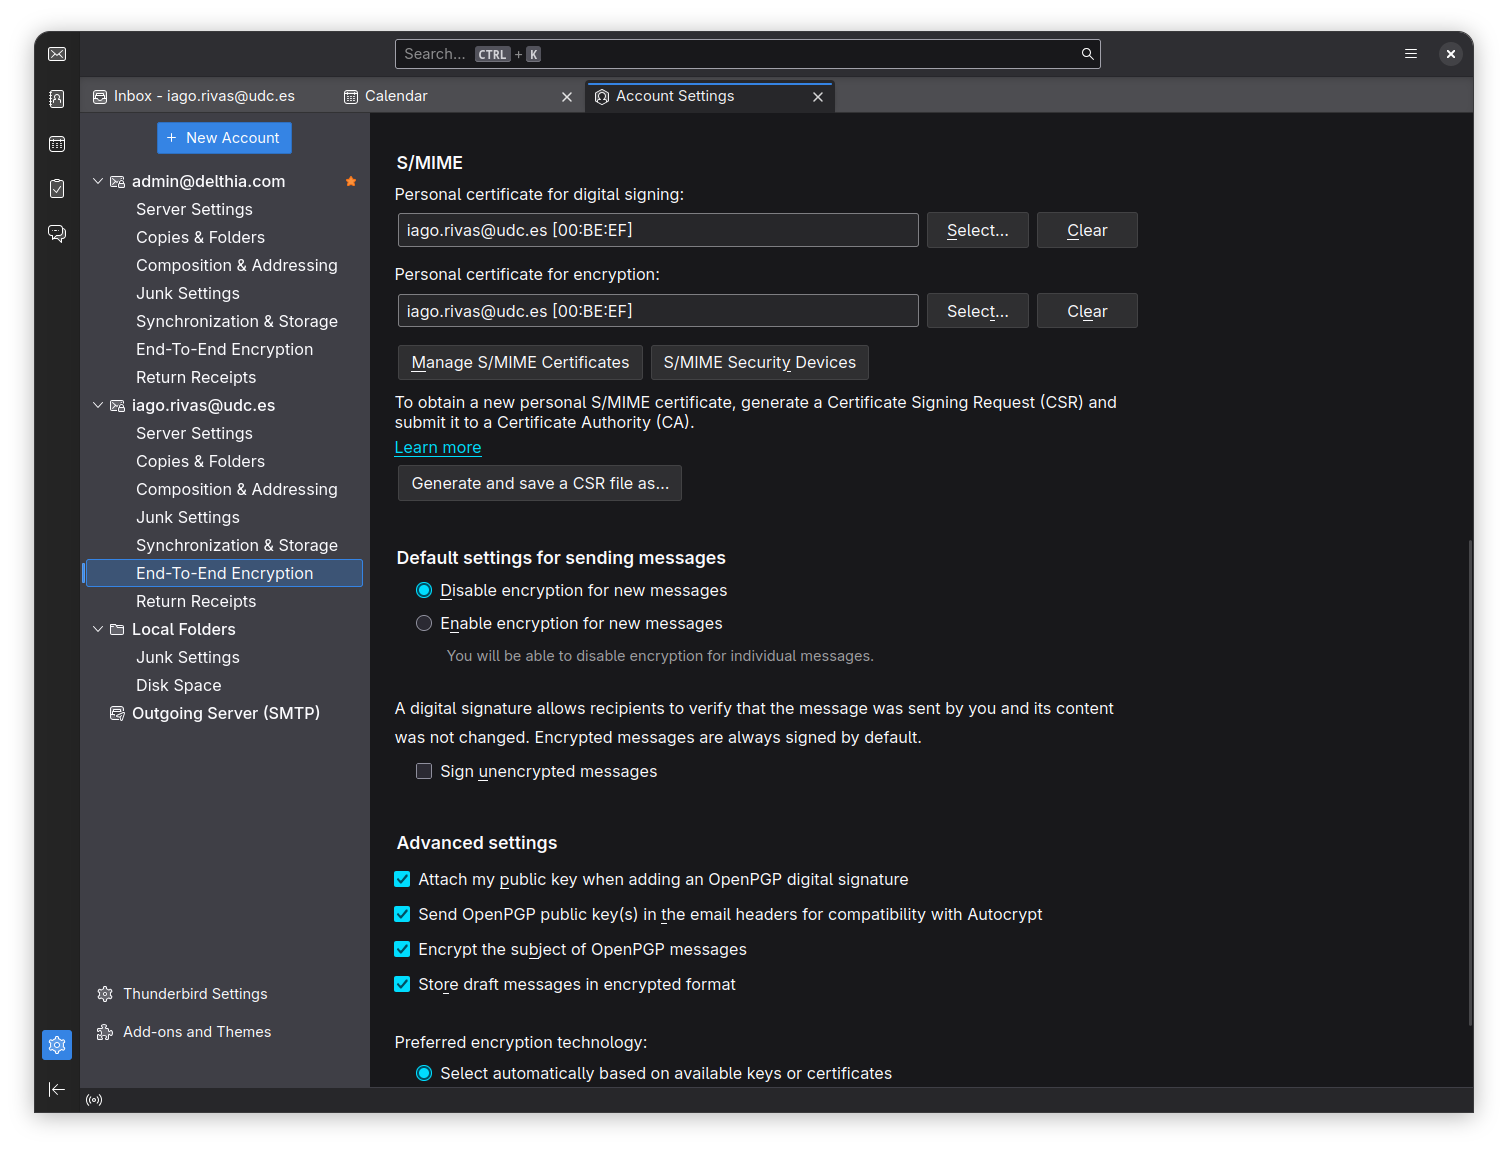
\includegraphics[width=\textwidth]{thunderbird-smime-configuracion.png}
    \caption{Ajustes de S/MIME en Thunderbird}
\end{figure}

Ahora podemos firmar y cifrar mensajes del mismo modo que cuando utilizábamos OpenPGP, seleccionando en el mismo desplegable la opción de S/MIME, en lugar de OpenPGP.

\begin{figure}[H]
    \centering
    \begin{subfigure}{.5\textwidth}
        \centering
        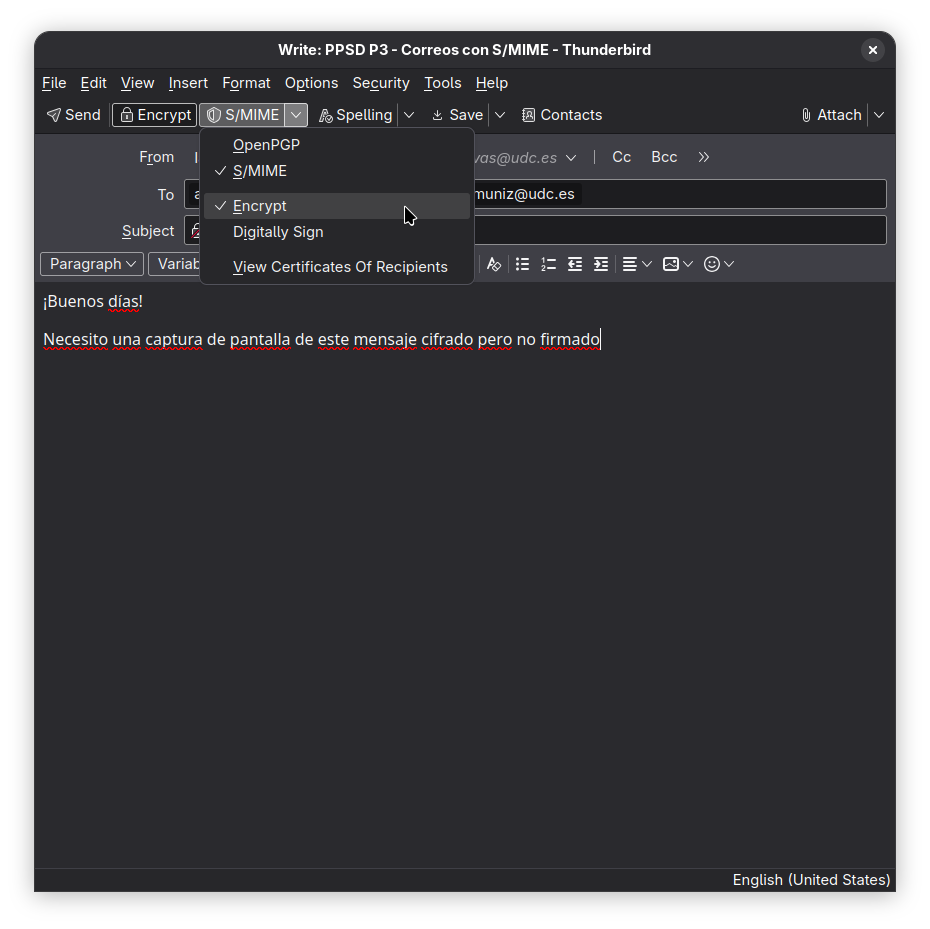
\includegraphics[width=\linewidth]{thunderbird-smime-cifrado.png}
        \caption{Envío del mensaje}
    \end{subfigure}%
    \begin{subfigure}{.5\textwidth}
        \centering
        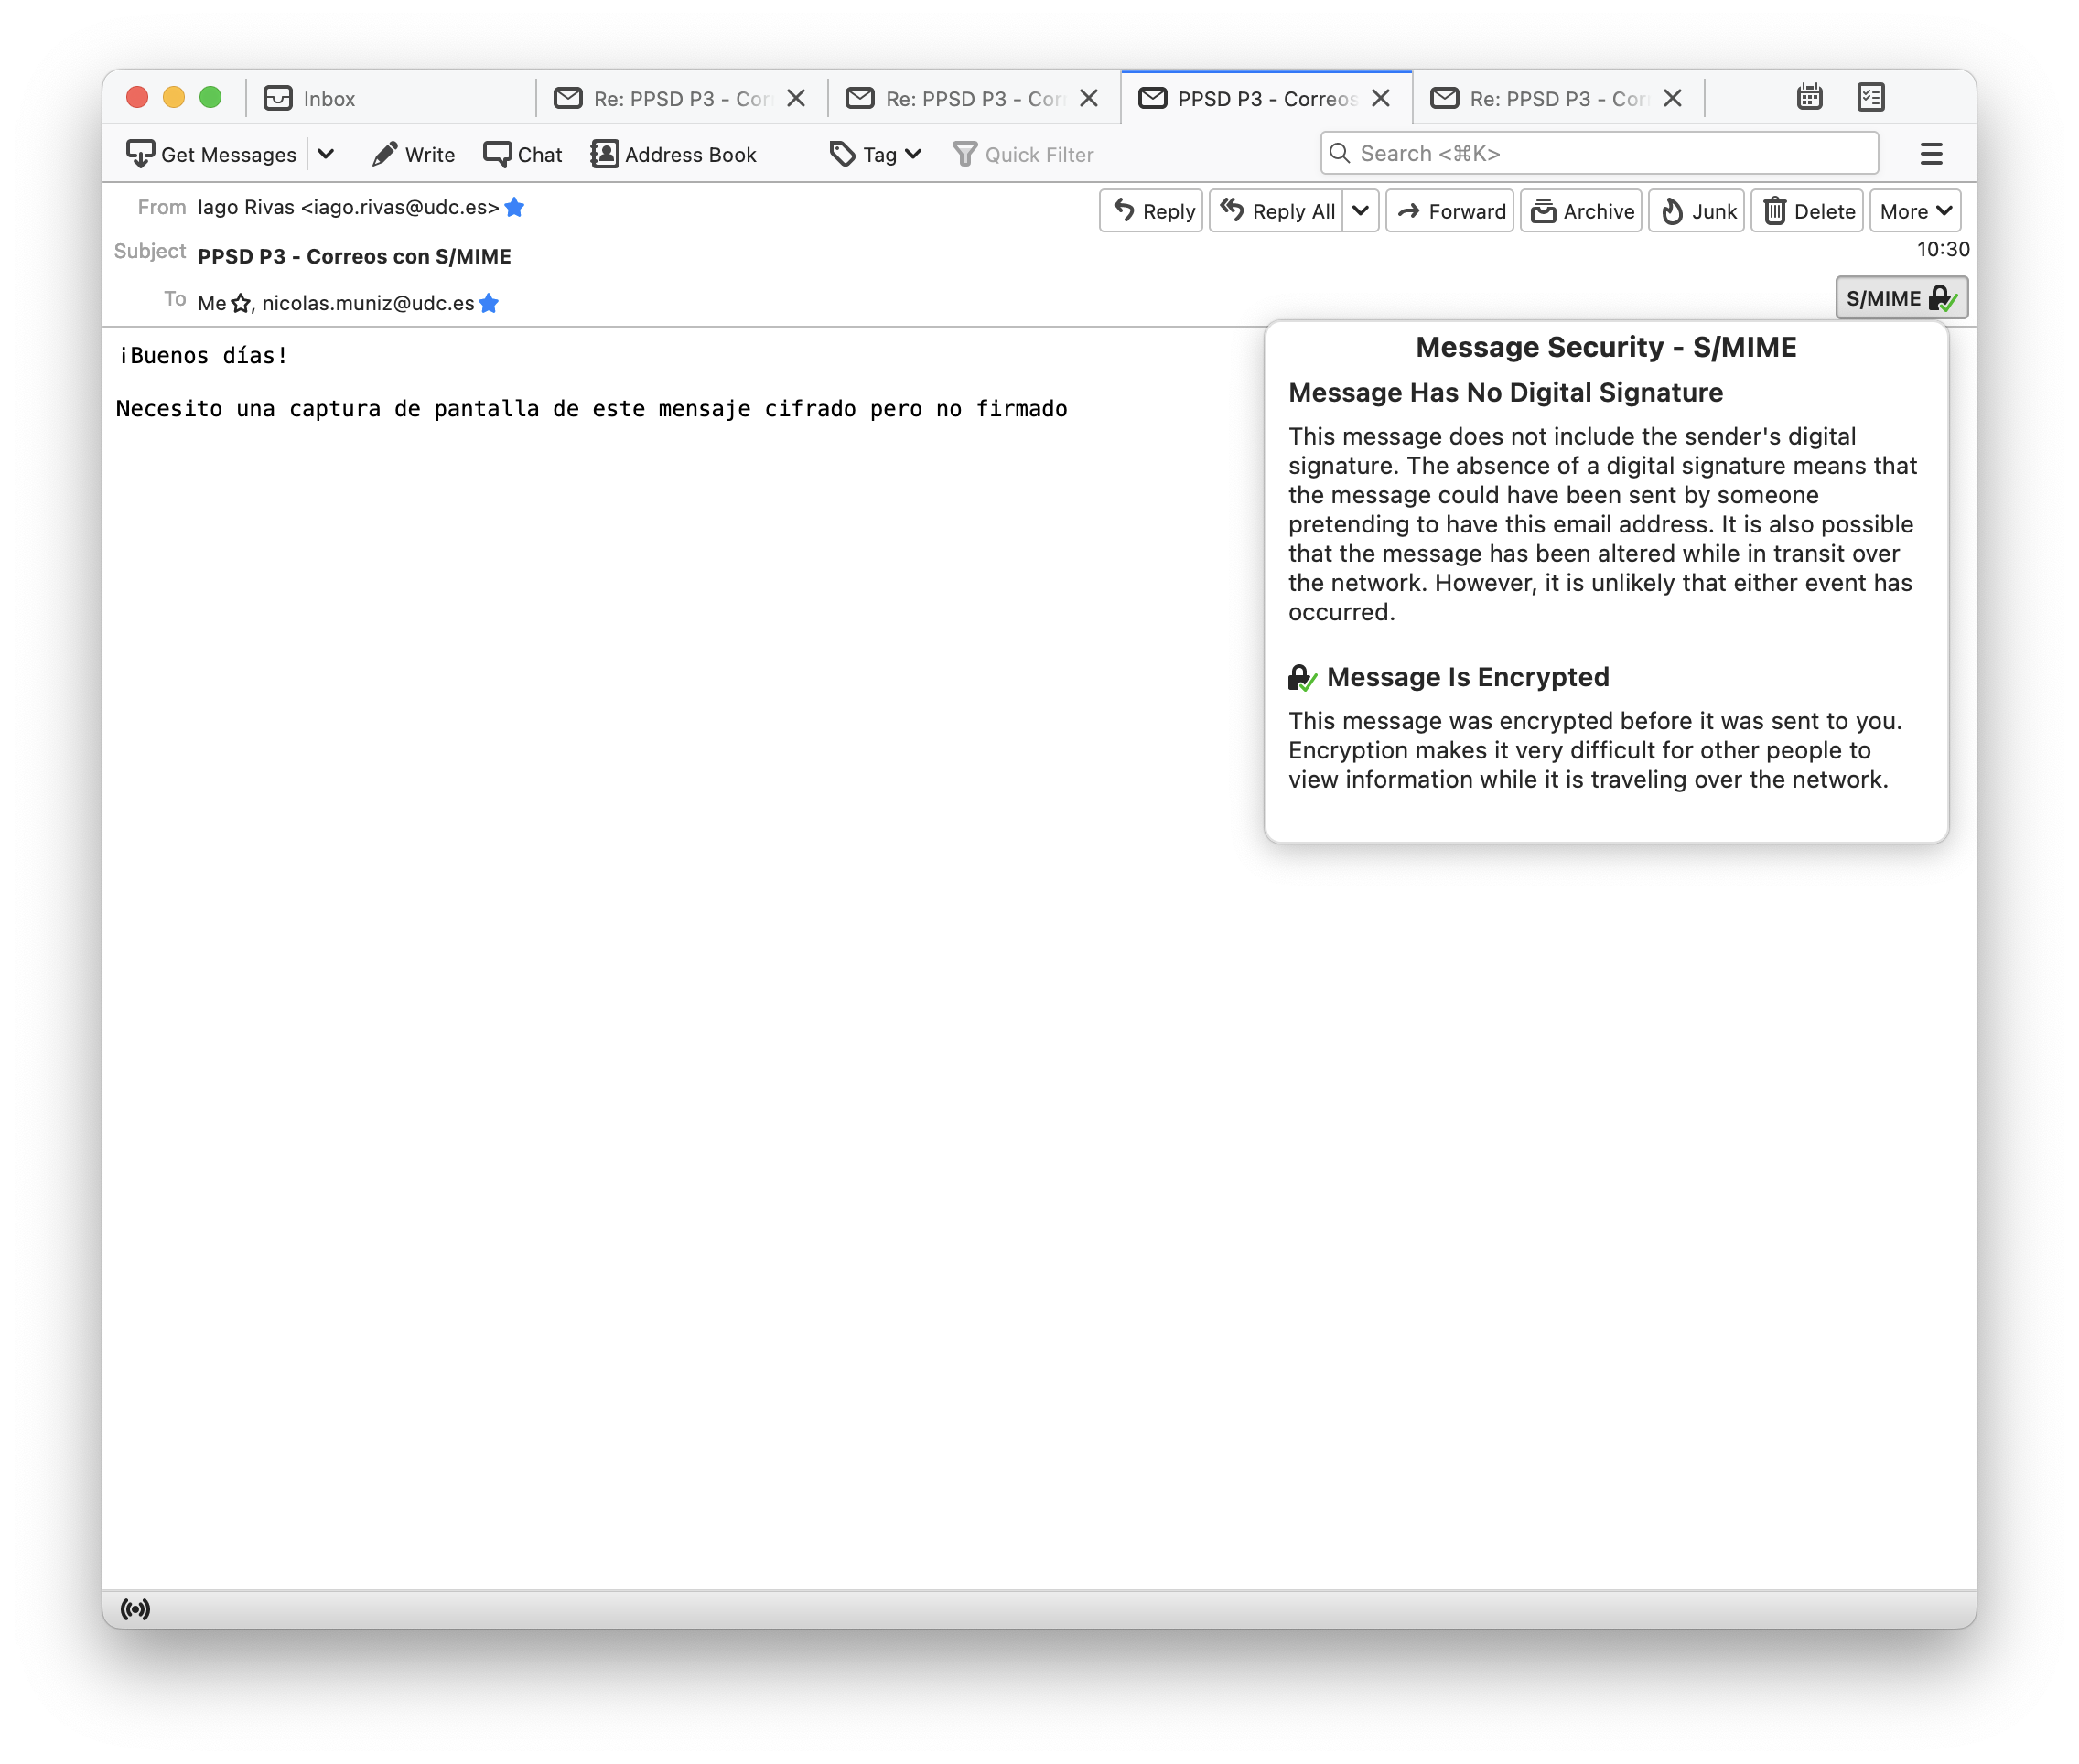
\includegraphics[width=1.2\linewidth]{thunderbird-smime-detalles-cifrado.png}
        \caption{Detalles del mensaje}
    \end{subfigure}
    \caption{Envío de un mensaje cifrado con S/MIME en Thunderbird}
\end{figure}

\begin{figure}[H]
    \centering
    \begin{subfigure}{.5\textwidth}
        \centering
        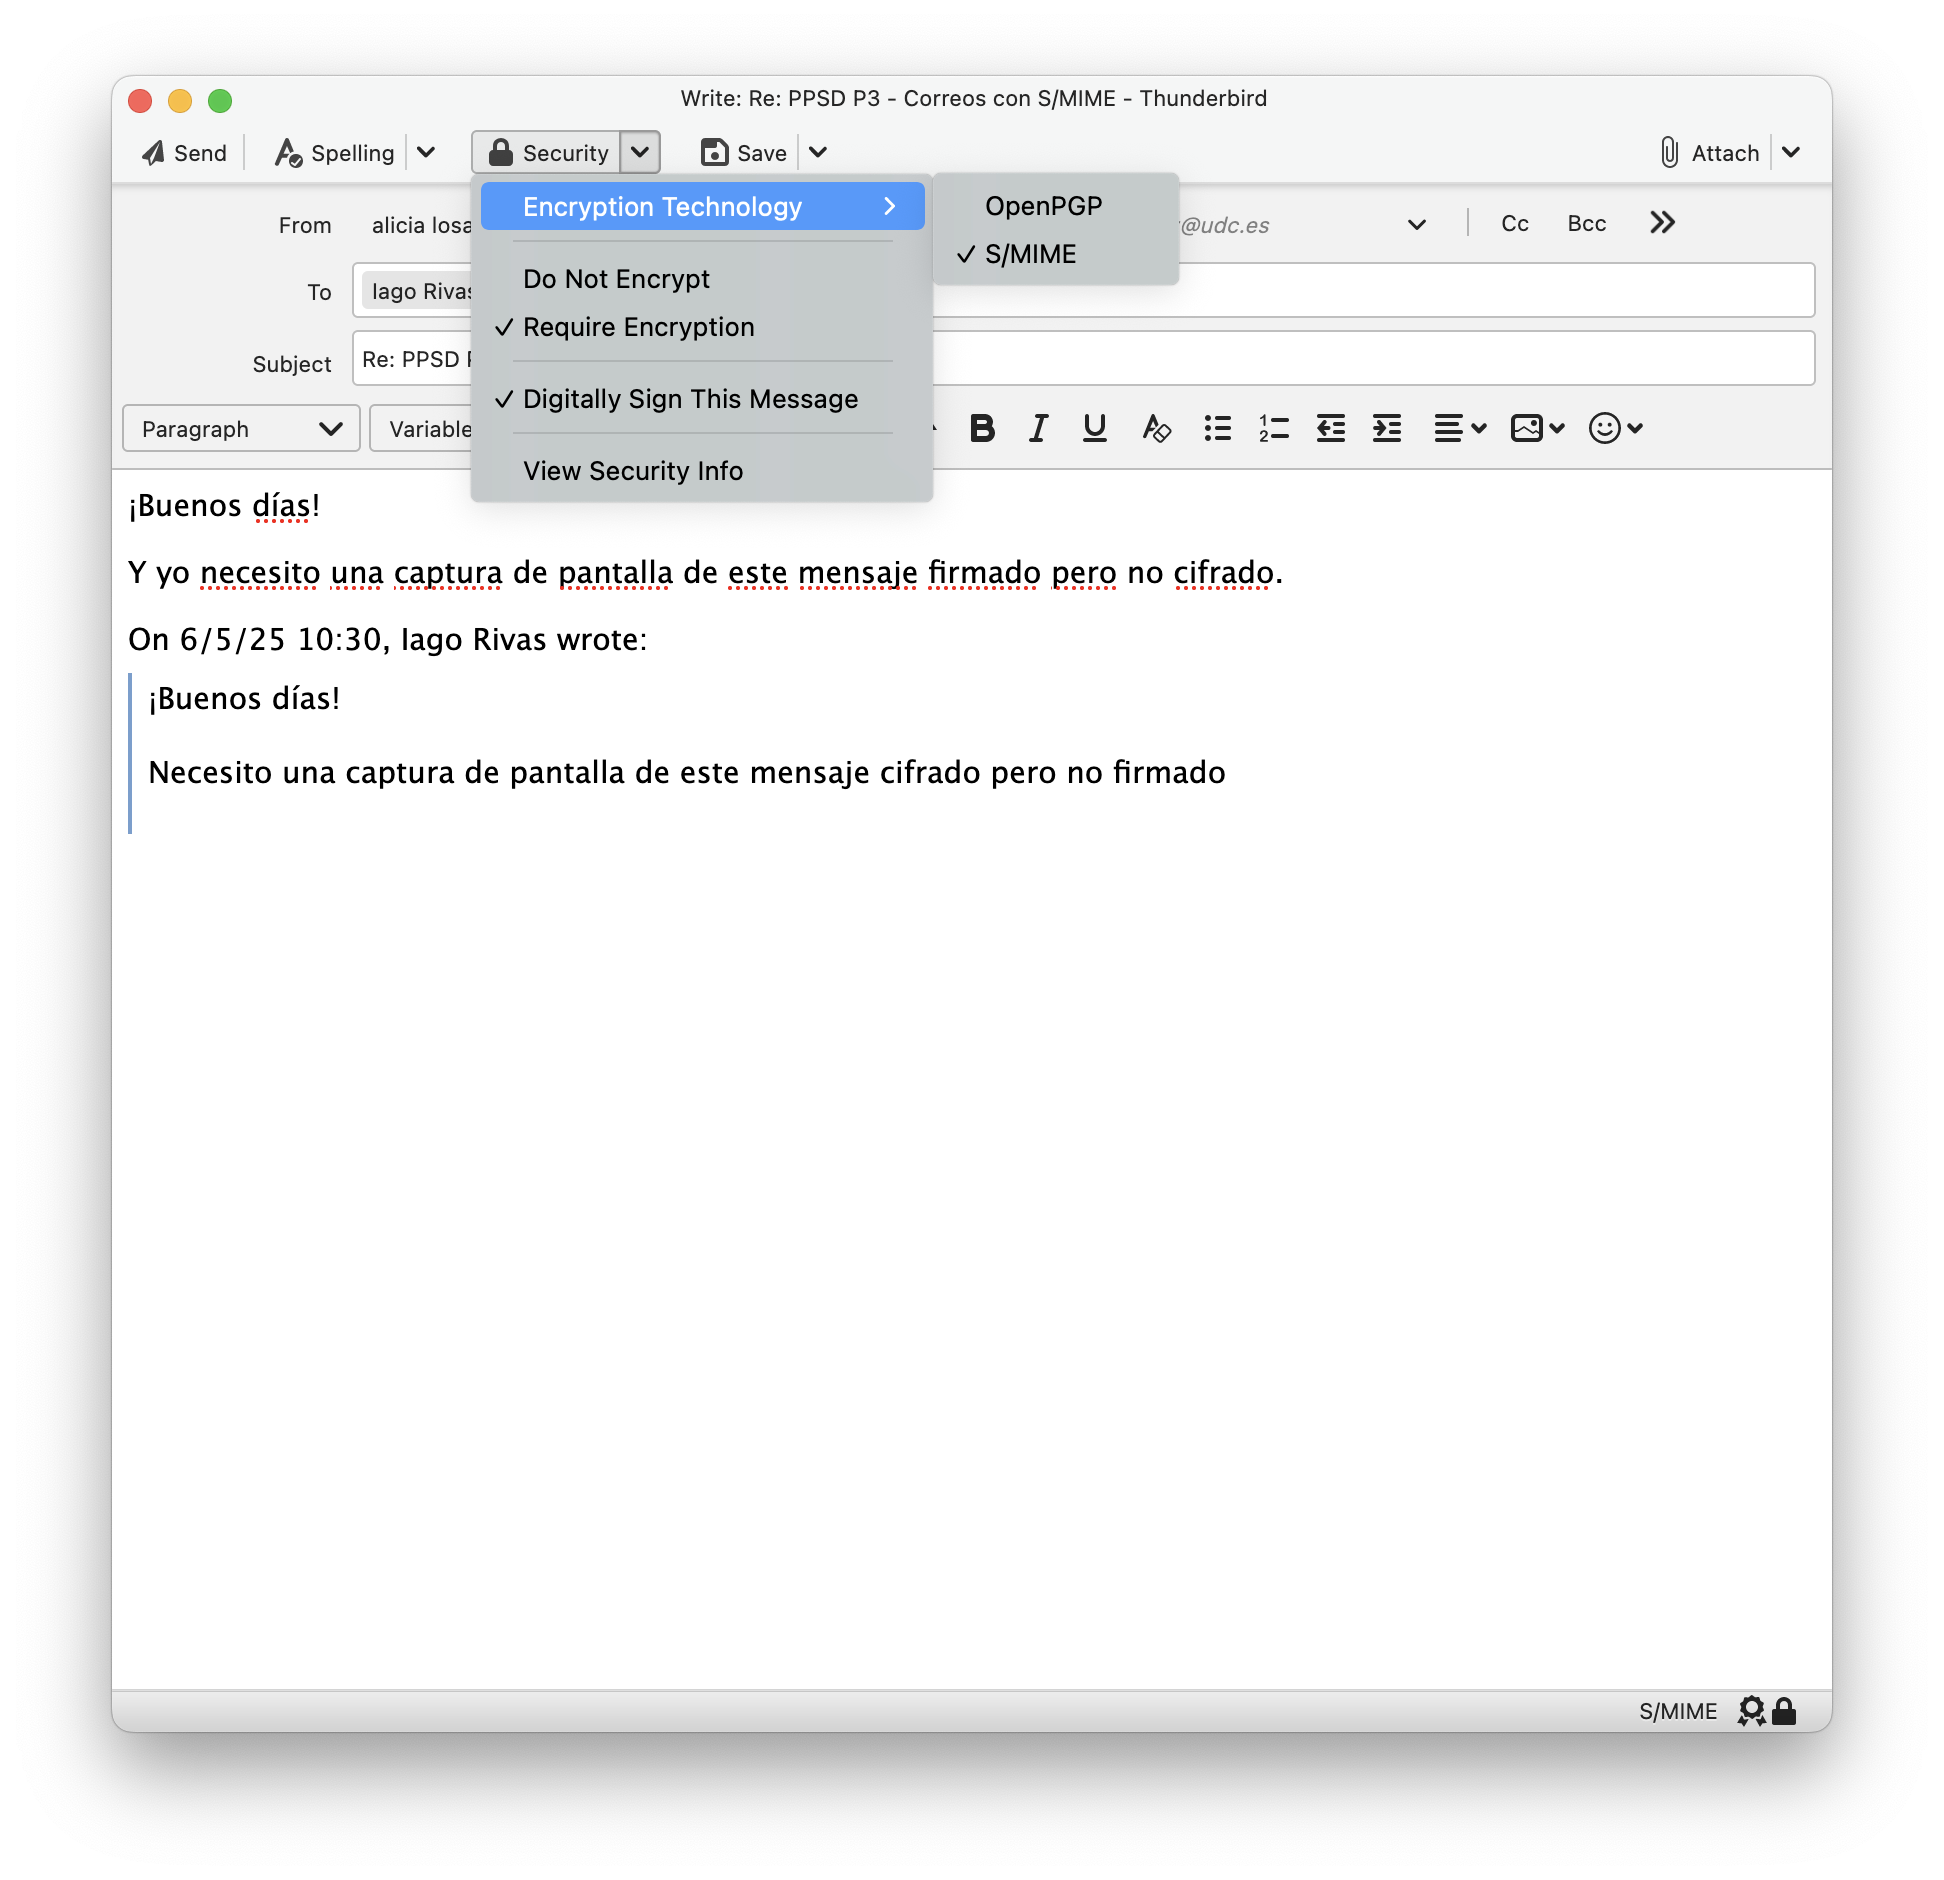
\includegraphics[width=\linewidth]{thunderbird-smime-firmado.png}
        \caption{Envío del mensaje}
    \end{subfigure}%
    \begin{subfigure}{.5\textwidth}
        \centering
        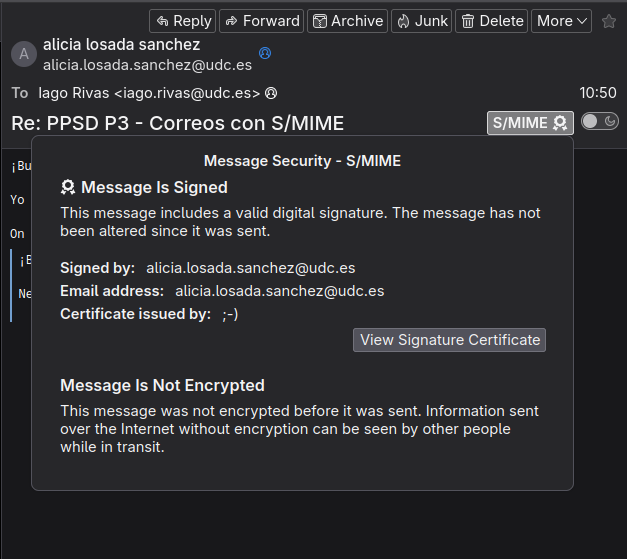
\includegraphics[width=1.2\linewidth]{thunderbird-smime-detalles-firmado.png}
        \caption{Detalles del mensaje}
    \end{subfigure}
    \caption{Envío de un mensaje firmado con S/MIME en Thunderbird}
\end{figure}

\begin{figure}[H]
    \centering
    \begin{subfigure}{.5\textwidth}
        \centering
        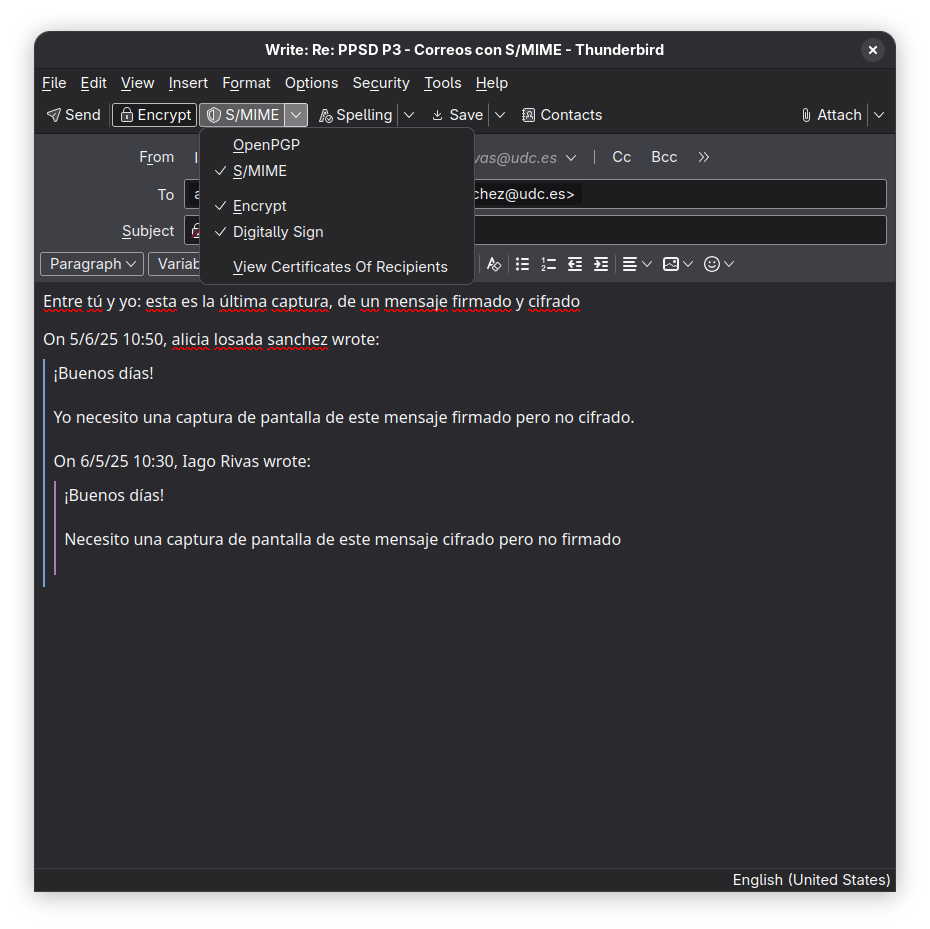
\includegraphics[width=\linewidth]{thunderbird-smime-firmado-cifrado.png}
        \caption{Envío del mensaje}
    \end{subfigure}%
    \begin{subfigure}{.5\textwidth}
        \centering
        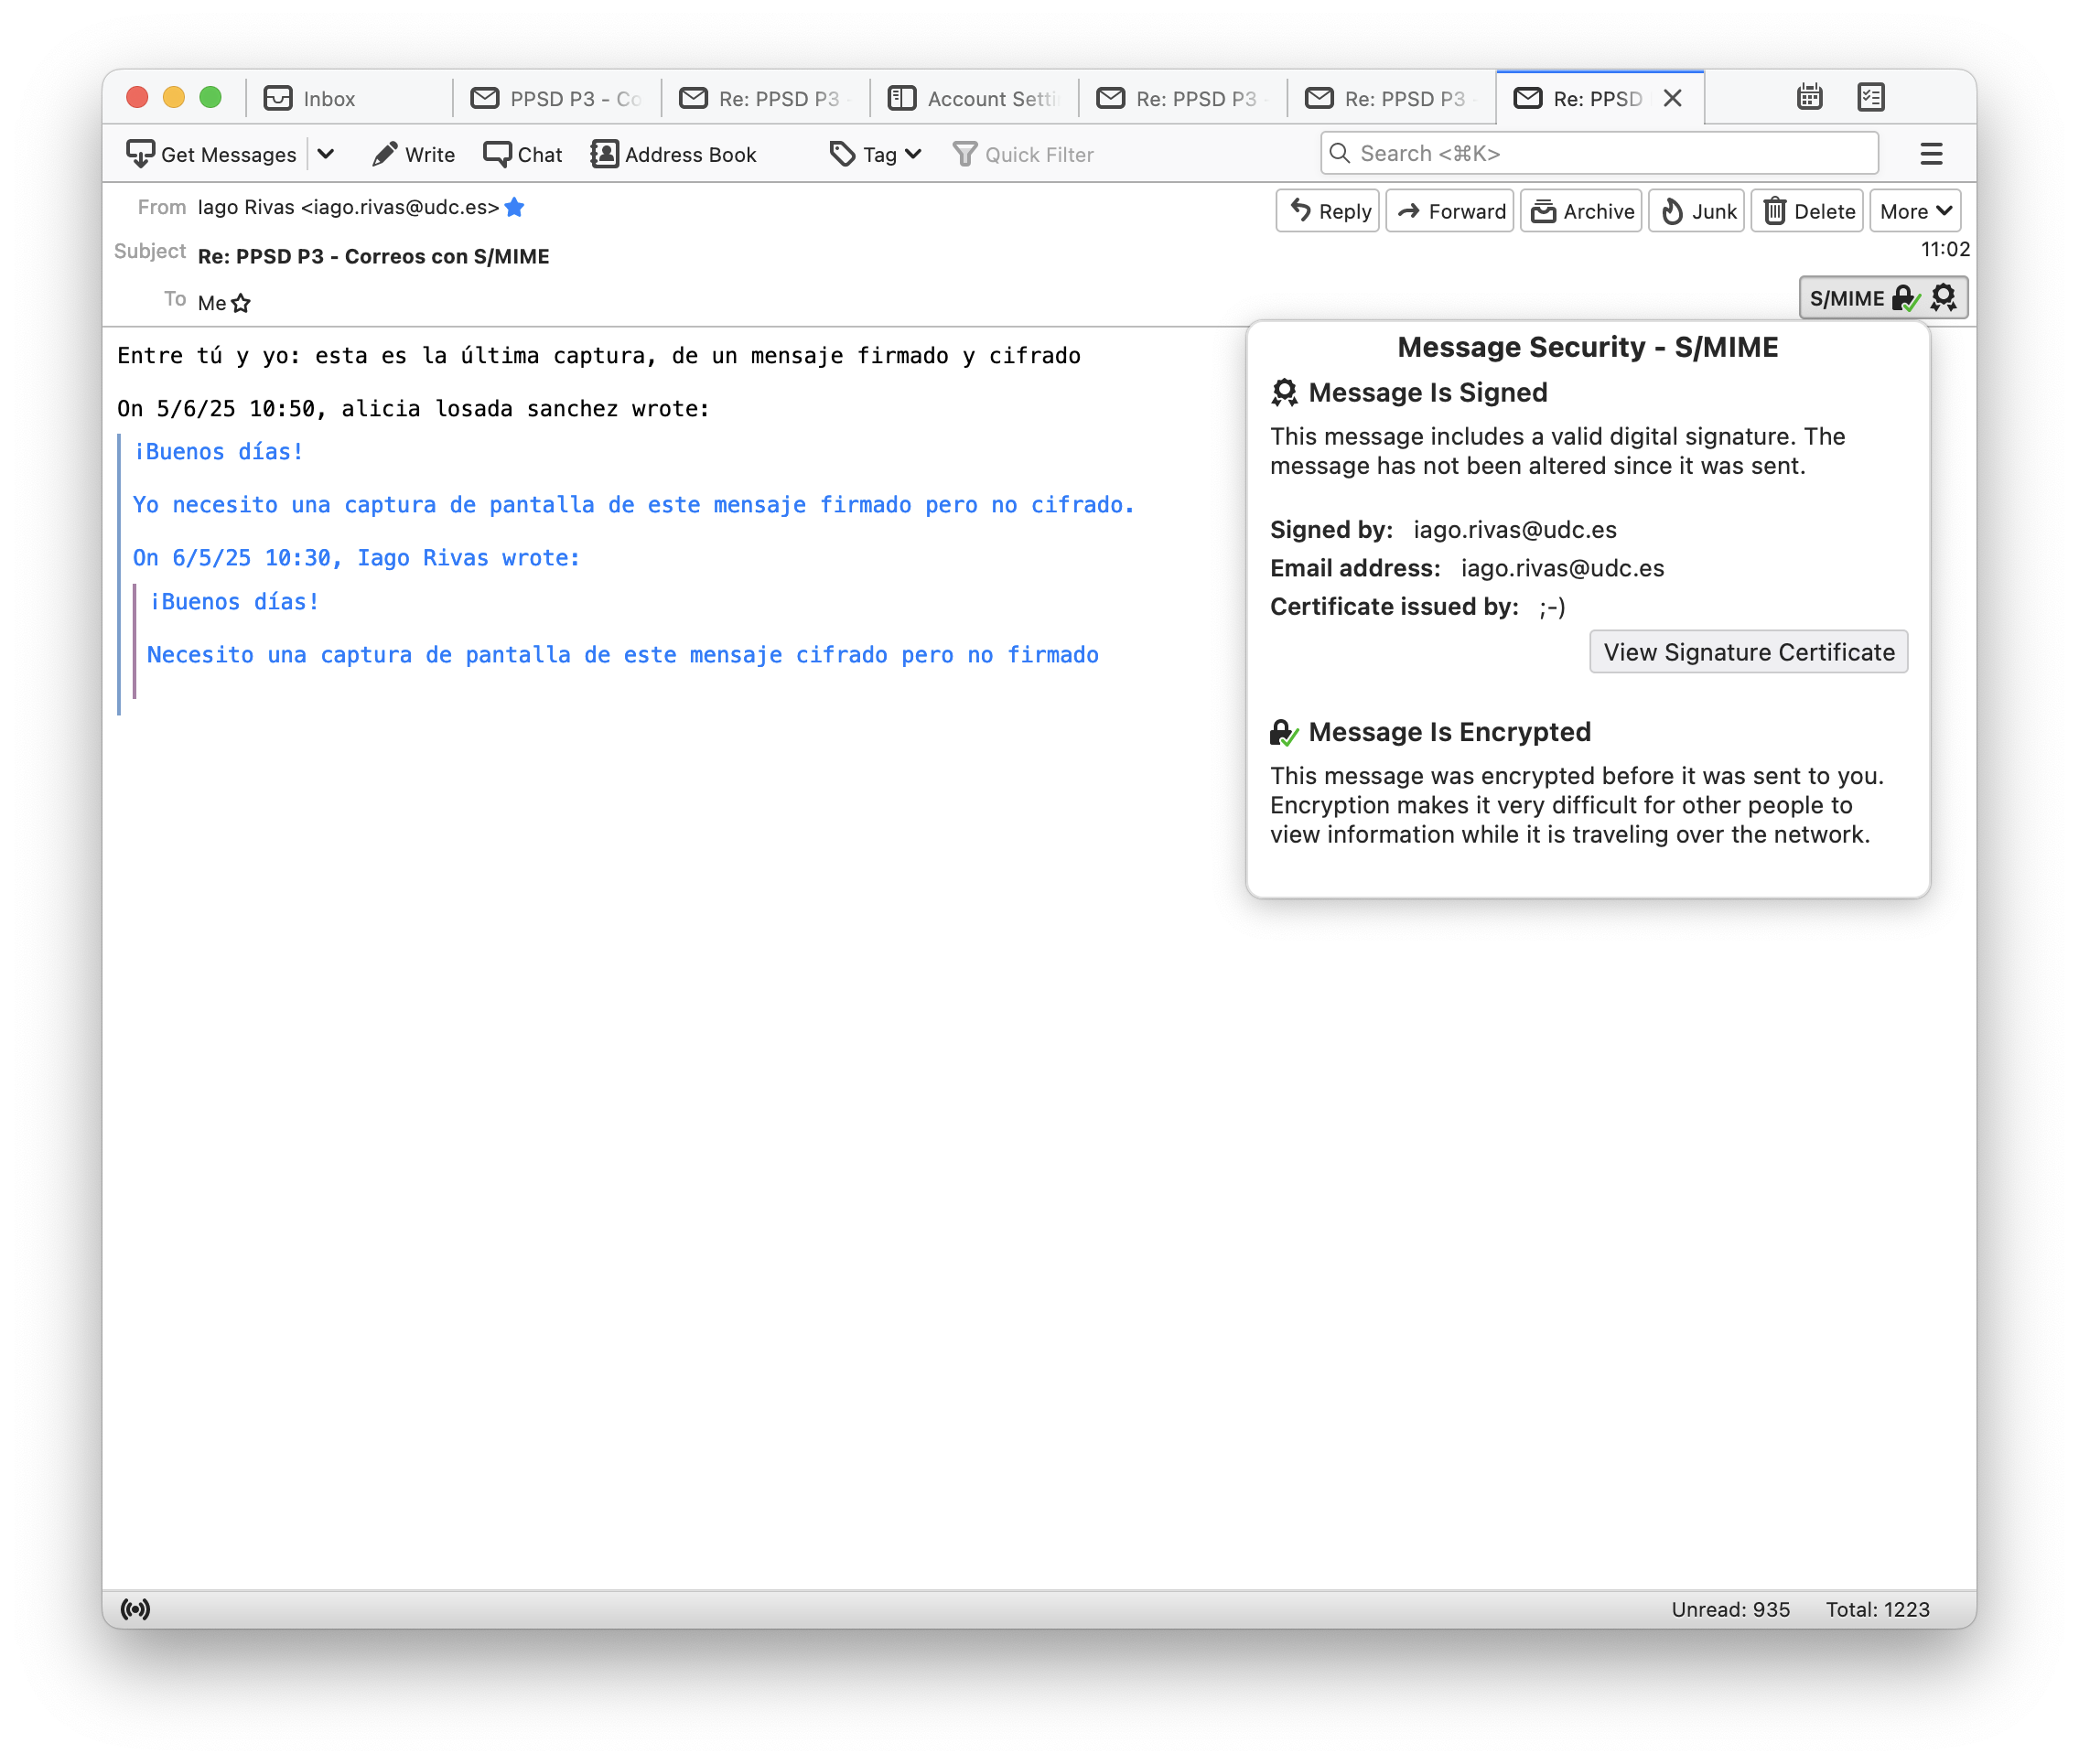
\includegraphics[width=1.2\linewidth]{thunderbird-smime-detalles-firmado-cifrado.png}
        \caption{Detalles del mensaje}
    \end{subfigure}
    \caption{Envío de un mensaje firmado y cifrado con S/MIME en Thunderbird}
\end{figure}